\chapter{予備実験}

本章では，第 4 章で述べた評価基盤を用いて実施した予備実験について述べる．5.1 節で目的を，5.2 節で設定を示し，5.3 節で結果を報告する．5.4 節で差の統計的な検証を行い，5.5 節で本章をまとめる．

本章に示す数値は，4.7 節で述べた採点処理の修正を反映したものである．修正前の値を用いた集計は本章には含まれない．

\section{実験の目的}

予備実験の目的は 2 つである．

第一に，構築した評価基盤が意図通りに動作することを確認することである．プロンプトの生成から指標の計算までが一貫して機能し，得られる数値が解釈可能であることを確かめる．

第二に，3 つの引き出し方式の間に較正の差が現れるかを把握することである．差の大きさが分かれば，本実験で必要な問題数の検討に使える．

予備実験は 1 モデル・1 領域での単一試行であり，結果から一般的な結論を導くことは意図していない．

\section{実験設定}

設定は表 3.3 に示した通りである．対象モデルは claude-sonnet-4-6，温度は0.0，データセットは日本語版 MGSM の 250 問である．3 方式それぞれについて250 問を実行し，合計 750 問分の応答を得た．Verb.2S は 1 問あたり 2 回のやりとりを行うため，API の呼び出しは設計上 1000 回となる．これは再試行を除いた回数であり，実際の呼び出し回数は記録していない．

\section{結果}

\subsection{主要な指標}

3 方式の結果を表 5.1 に示す．

\begin{table}[htbp]
\centering
\small
\caption{3 方式の比較（日本語版 MGSM，250 問）}
\label{tab:5.1}
\scalebox{0.93}{
\begin{tabular}{|l|l|l|l|l|l|l|l|l|}
\hline
方式 & 採点対象 & 正答率 & ECE & Brier & AUROC & REL & RES & UNC \\
\hline
Verb.1S & 248 & 215/250 = 86.0\% & 0.0712 & 0.0978 & 0.738 & 0.0115 & 0.0287 & 0.1154 \\
Verb.2S & 250 & 221/250 = 88.4\% & 0.0438 & 0.0785 & 0.797 & 0.0070 & 0.0284 & 0.1025 \\
Ling.1S & 250 & 195/250 = 78.0\% & 0.1266 & 0.1733 & 0.629 & 0.0170 & 0.0153 & 0.1716 \\
\hline
\end{tabular}
}
\end{table}

正答率の分母は全 250 問である．一方 ECE，Brier Score，AUROC，Murphy 分解は確信度が取得できた問題のみで計算しており，その件数を「採点対象」列に示した．確信度の取得に失敗したのは Verb.1S の 2 問（mgsm\_ja\_081，mgsm\_ja\_142）のみである．

3.4.3 項で述べたとおり，REL − RES + UNC は区間に集約した予測に対するBrier Score に対応し，表中の Brier Score とは一般に一致しない．実際の差はVerb.1S で −0.0003，Verb.2S で −0.0026 であった．Ling.1S では確信度が区間ごとに 1 つの値しかとらないため差は 0 である．

正答率，ECE，Brier Score，AUROC，REL の点推定では Verb.2S が最良であった．RES の点推定は Verb.1S が最も高い（0.0287 に対し Verb.2S は 0.0284）．いずれも点推定の比較であり，統計的な検証は 5.4 節で行う．

\subsection{確信度の分布}

確信度の分布を図 5.1 に示す（\texttt{fig2\_\allowbreak{}confidence.\allowbreak{}png}，各方式の採点対象件数）．3 方式のいずれにおいても，確信度が 0.9 以上の区間に偏っている．該当する件数は Verb.1S が 248 件中 225 件，Verb.2S が 250 件中 217 件，Ling.1S が250 件中 203 件である．

Ling.1S では 5 段階のうち 4 段階が使われた．内訳は「ほぼ確実」が 203 件，「かなり自信がある」が 36 件，「どちらともいえない」が 9 件，「あまり自信がない」が 2 件であり，「ほとんどわからない」は 1 件も選ばれなかった．最上位が全体の 81.2\% を占める．

\begin{figure}[htbp]
\begin{center}
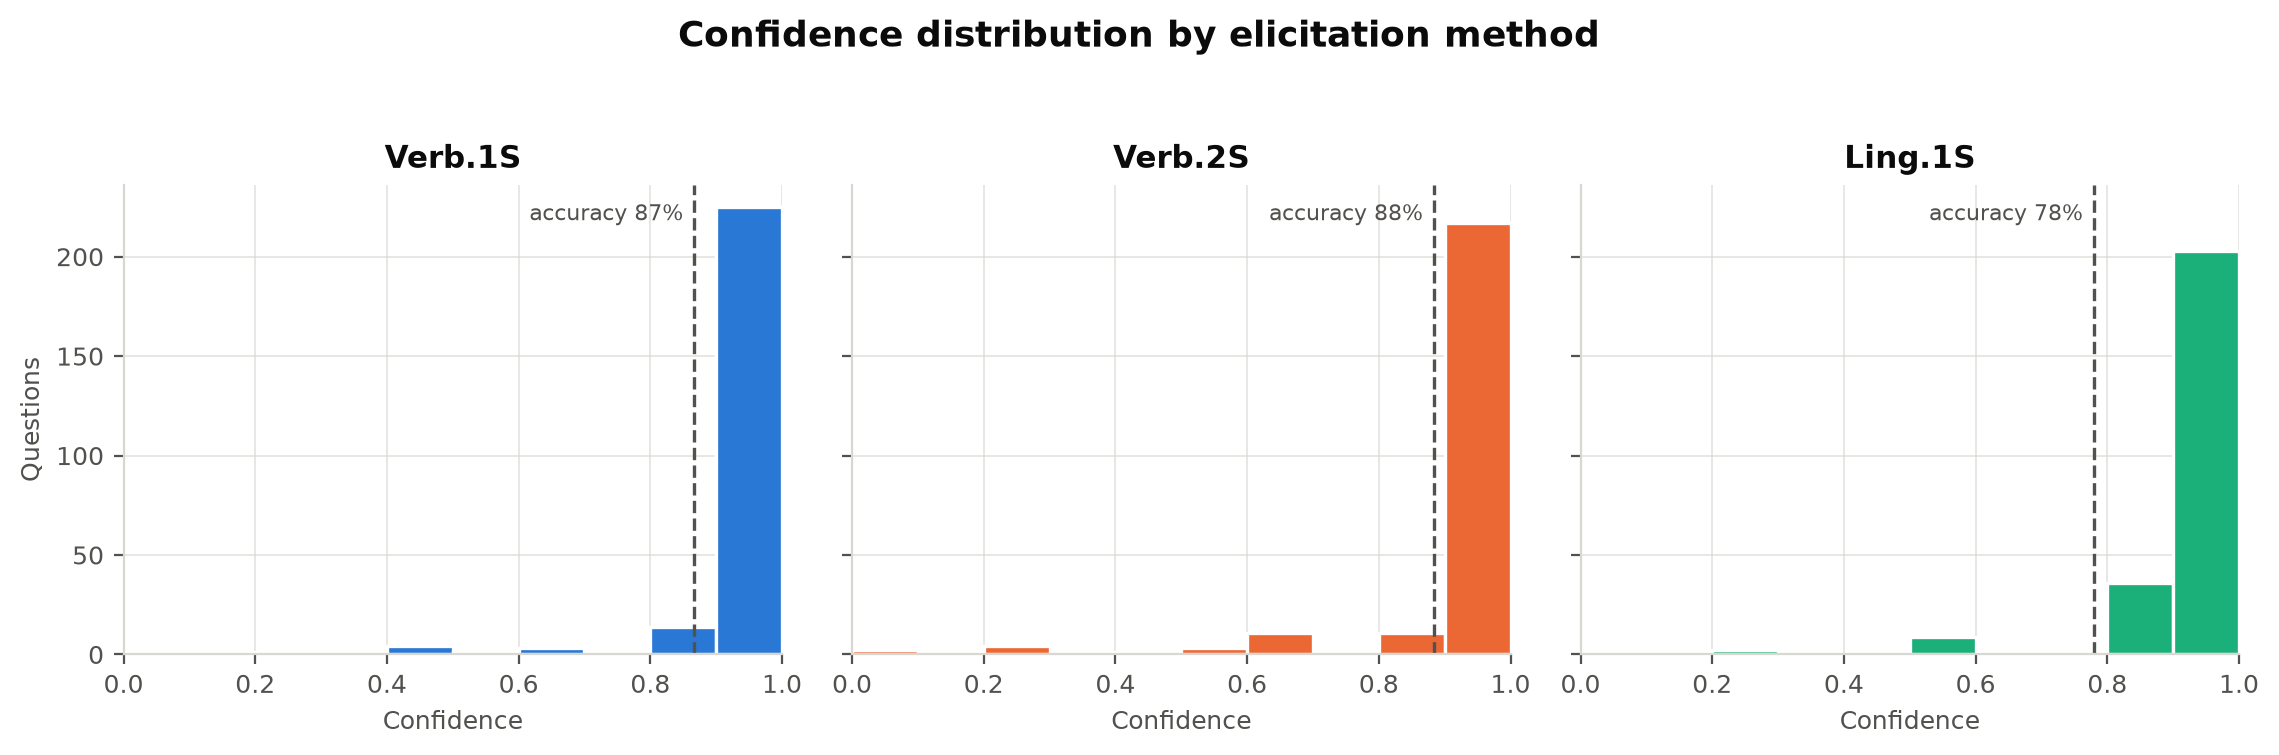
\includegraphics[width=14cm]{./figure/confidence-distribution.png}
\caption{確信度の分布（方式別）}
\label{fig:5.1}
\end{center}
\end{figure}

平均確信度と平均正答率を表 5.2 に示す．いずれも採点対象の件数を分母とする．

\begin{table}[htbp]
\centering
\small
\caption{平均確信度と平均正答率（採点対象のみ）}
\label{tab:5.2}
\begin{tabular}{|l|l|l|l|l|}
\hline
方式 & 採点対象 & 平均確信度 & 平均正答率 & 差 \\
\hline
Verb.1S & 248 & 0.938 & 0.867 & +0.071 \\
Verb.2S & 250 & 0.921 & 0.884 & +0.037 \\
Ling.1S & 250 & 0.907 & 0.780 & +0.127 \\
\hline
\end{tabular}
\end{table}

3 方式とも平均確信度は 0.91 から 0.94 の範囲にあり，方式による差は小さい．差はいずれも正であり，モデルは実際の正答率より高い確信度を表明している．方式によって大きく変化したのは確信度ではなく正答率の側である．

\subsection{信頼度ダイアグラム}

確信度と正答率の対応を図 5.2 に示す（\texttt{fig1\_\allowbreak{}reliability.\allowbreak{}png}）．対角線は完全な較正に相当し，これより下側にある点は，その確信度帯において確信度が正答率を上回っていることを示す．

\begin{figure}[htbp]
\begin{center}
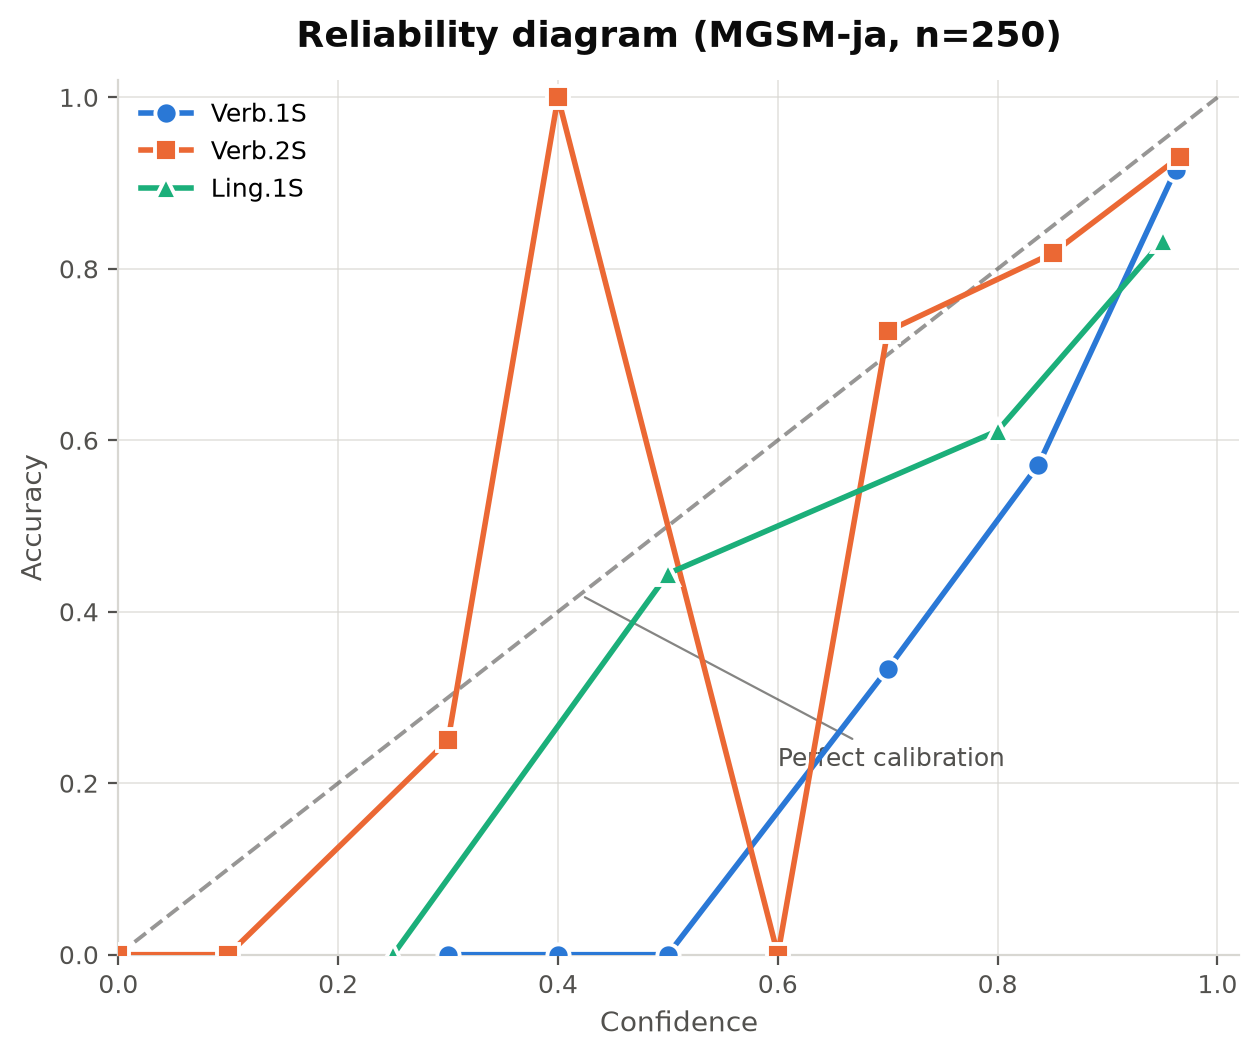
\includegraphics[width=11cm]{./figure/reliability-diagram.png}
\caption{信頼度ダイアグラム}
\label{fig:5.2}
\end{center}
\end{figure}

10 区間のうち標本が存在する区間は，Verb.1S で 6 個，Verb.2S で 8 個，Ling.1S で 4 個である．低確信度側には 1 件ないし数件しか含まれない区間があり，そこでの区間正答率は少数の問題に左右される．折れ線はこの違いを表現しないため，低確信度帯の点を高確信度帯の点と同じ重みで読むことはできない．

\section{差の統計的検証}

\subsection{検証の方法}

表 5.1 の差が標本の揺らぎで説明できるかを確かめるため，問題の復元抽出による信頼区間を求めた．3 方式すべてで確信度が取得できた 248 問を対象とし，5000 回の再抽出を行った．4.6 節で述べたとおり，3 方式には同じ添字を適用する対応のある設計とした．

対象が 248 問に揃うため，本節の点推定は表 5.1 の値とわずかに異なる．

なお，以下に示すのは 18 通りの比較それぞれに対する個別の 95\% 信頼区間であり，全体を同時に 95\% で保証するものではない．多重比較の調整は行っておらず，探索的な分析として扱う．

\subsection{各方式の指標の信頼区間}

各指標の 95\% 信頼区間を表 5.3 に示す（共通 248 問）．

\begin{table}[htbp]
\centering
\small
\caption{各指標の 95\% 信頼区間（共通 248 問）}
\label{tab:5.3}
\begin{tabular}{|l|l|l|l|}
\hline
指標 & Verb.1S & Verb.2S & Ling.1S \\
\hline
ECE & 0.071 [0.036, 0.110] & 0.043 [0.022, 0.086] & 0.123 [0.080, 0.175] \\
Brier & 0.098 [0.066, 0.131] & 0.078 [0.052, 0.109] & 0.171 [0.133, 0.213] \\
AUROC & 0.738 [0.625, 0.841] & 0.792 [0.668, 0.897] & 0.626 [0.556, 0.697] \\
REL & 0.012 [0.005, 0.027] & 0.007 [0.003, 0.017] & 0.016 [0.007, 0.034] \\
RES & 0.029 [0.013, 0.051] & 0.026 [0.011, 0.048] & 0.013 [0.004, 0.031] \\
正答率 & 0.867 [0.823, 0.907] & 0.887 [0.847, 0.923] & 0.786 [0.734, 0.835] \\
\hline
\end{tabular}
\end{table}

\subsection{方式間の差}

方式間の差の信頼区間を表 5.4 に示す．区間が 0 を含まない場合，その差は標本の揺らぎでは説明しにくい．

\begin{table}[htbp]
\centering
\small
\caption{方式間の差の 95\% 信頼区間（共通 248 問）}
\label{tab:5.4}
\begin{tabular}{|l|l|l|l|l|}
\hline
指標 & 比較 & 差 & 95\% 信頼区間 & 判定 \\
\hline
ECE & Verb.1S − Verb.2S & +0.029 & [−0.014, +0.054] & 0 を含む \\
ECE & Verb.1S − Ling.1S & −0.052 & [−0.097, −0.012] & 0 を含まない \\
ECE & Verb.2S − Ling.1S & −0.080 & [−0.120, −0.031] & 0 を含まない \\
Brier & Verb.1S − Verb.2S & +0.019 & [−0.007, +0.047] & 0 を含む \\
Brier & Verb.1S − Ling.1S & −0.073 & [−0.109, −0.038] & 0 を含まない \\
Brier & Verb.2S − Ling.1S & −0.092 & [−0.129, −0.058] & 0 を含まない \\
AUROC & Verb.1S − Verb.2S & −0.054 & [−0.145, +0.030] & 0 を含む \\
AUROC & Verb.1S − Ling.1S & +0.112 & [+0.012, +0.211] & 0 を含まない \\
AUROC & Verb.2S − Ling.1S & +0.166 & [+0.048, +0.274] & 0 を含まない \\
REL & Verb.1S − Verb.2S & +0.005 & [−0.007, +0.017] & 0 を含む \\
REL & Verb.1S − Ling.1S & −0.004 & [−0.019, +0.009] & 0 を含む \\
REL & Verb.2S − Ling.1S & −0.009 & [−0.024, +0.003] & 0 を含む \\
RES & Verb.1S − Verb.2S & +0.003 & [−0.014, +0.019] & 0 を含む \\
RES & Verb.1S − Ling.1S & +0.015 & [−0.001, +0.034] & 0 を含む \\
RES & Verb.2S − Ling.1S & +0.013 & [−0.006, +0.033] & 0 を含む \\
正答率 & Verb.1S − Verb.2S & −0.020 & [−0.052, +0.012] & 0 を含む \\
正答率 & Verb.1S − Ling.1S & +0.081 & [+0.036, +0.125] & 0 を含まない \\
正答率 & Verb.2S − Ling.1S & +0.101 & [+0.056, +0.145] & 0 を含まない \\
\hline
\end{tabular}
\end{table}

全 18 通りの比較のうち，8 通りで区間が 0 を含まなかった．

\subsection{検証から言えること}

検証の結果，主張できることは 3 点に限られる．

\textbf{Ling.1S は他の 2 方式より ECE，Brier Score，AUROC，正答率で劣る．}この 4 指標において，Ling.1S と他の 2 方式との差はいずれも区間が 0 を含まなかった．

\textbf{REL と RES では差を検出できなかった．} REL は 3 通りの比較すべてで区間が0 を含む．したがって，Ling.1S の較正が他の 2 方式より劣ることを REL の水準で示すことはできていない．RES も同様である．ただし AUROC では Ling.1S との差が検出されているため，識別に関わる性質全般について差がないとは言えない．

\textbf{Verb.1S と Verb.2S の差は判定できない．} 6 指標すべてで区間が 0 を含んだ．したがって，2 段階方式が 1 段階方式より優れているとは言えない．ただしこれは差が存在しないことを示すものでもない．今回の標本では検出できなかった，というのが正確な表現である．必要な標本数を見積もるには，実用上意味のある差の大きさを先に定める必要がある．

\section{本章のまとめ}

本章では予備実験の設定と結果を示した．評価基盤は一貫して動作し，4 つの指標すべてが計算できた．方式間の比較では，Ling.1S が他の 2 方式より ECE，Brier Score，AUROC，正答率において劣ることが確認された一方，REL と RES では差を検出できず，Verb.1S と Verb.2S の差はどの指標でも判定できなかった．また 3 方式に共通して，確信度が 0.9 以上に偏る傾向が観察された．次章ではこの偏りの意味と，評価指標の読み方について考察する．
